\documentclass{beamer}

\usepackage[utf8]{inputenc}
\usepackage[T1]{fontenc}
\usepackage{ngerman}
\usepackage{tcolorbox}
\usepackage{amsmath,amsfonts,amssymb}	 % math. Symbole 
\usepackage{textcomp}			         % Sonderzeichen
\usepackage{natbib}
\usepackage{listings}                    % Code blocks
\usepackage{multicol}

\setbeamertemplate{itemize items}{>>}
\setbeamertemplate{itemize subitem}[square]
\setbeamertemplate{itemize subsubitem}[ball]

\title{POSIX}
\subtitle{Portable Operating System Interface}
\author{
	ptrLx
}
\date{15. Dezember 2021}

\usetheme{Madrid}
\usecolortheme{crane}

\begin{document}
\frame {
    \titlepage
}

\frame {
    \frametitle{Definition}
    \begin{tcolorbox}
        Das Portable Operating System Interface ist eine gemeinsam vom IEEE und der Open Group für Unix entwickelte standardisierte Programmierschnittstelle, welche die Schnittstelle zwischen Anwendungssoftware und Betriebssystem darstellt. (ISO/IEC/IEEE 9945)
    \end{tcolorbox}
}

\frame {
    \frametitle{Überblick}
    \begin{itemize}
        \item \textbf{Basis-Definitionen}\\
              Eine Liste der im Standard benutzten Konventionen, Definitionen und Konzepte
        \item \textbf{System-Schnittstelle}\\
              Die C-Systemaufrufe und dazugehörige Header-Dateien\\
        \item \textbf{Kommandozeileninterpreter und Hilfsprogramme}\\
              Eine Liste der Hilfsprogramme und der Kommandozeileninterpreter\\
        \item \textbf{Erklärungen} \\
              Erläuterungen über den Standard
    \end{itemize}
}

\frame{
    \frametitle{Posix C API}
    Ergänzung der Stdlib um Funktionalitäten wie:
    \begin{itemize}
        \item Threads / Prozesse / Signale
        \item Netzwerk Funktionalitäten (Sockets)
        \item Reguläre Ausdrücke
        \item Datei / Dateisystem Funktionalitäten
        \item Erweiterte Typen
        \item Benutzer- / Gruppenverwaltung
        \item Zeit / Datum
    \end{itemize}
    Vollständige Spezifikation: \url{https://pubs.opengroup.org/onlinepubs/9699919799/functions/contents.html}
}

\frame{
    \frametitle{Environment Variablen}
    \begin{itemize}
        \item Environment Variablen sind Variablen die ihre Gültigkeit in einer Shell haben und darin ausgeführten Programmen zur Verfügung stehen. Sie geben Aufschluss über die Umgebung des Systems (z.B. Betriebssystem, Benutzer, Konfigurationen ...).
        \item Wichtige Variablen sind:
              \begin{itemize}
                  \item \$PATH: Beinhaltet Verzeichnisse, in denen Programme liegen, die ohne Pfadangabe gefunden werden sollen
                  \item \$HOME: Benutzerverzeichnis
                  \item \$SHELL: Bevorzugte Shell
              \end{itemize}
        \item In vielen Systemen werden sie genutzt um bestimmte Konfigurationsparameter einzustellen (z.B. stage, Hostname des Datenbank-Servers, ...)
    \end{itemize}
    Vollständige Spezifikation: \url{https://pubs.opengroup.org/onlinepubs/9699919799/basedefs/V1_chap08.html}
}

\frame{
    \frametitle{CLI utilities}
    Wichtige CLI utilities sind:
    \begin{multicols*}{2}
        \begin{itemize}
            \item echo: String ausgeben
            \item cd: Verzeichnis wechseln
            \item ls: Verzeichnisinhalt anzeigen
            \item mkdir: Verzeichnis erstellen
            \item mv: Datei verschieben
            \item rm: Datei löschen
            \item rmdir: Ordner löschen
            \item pwd: Pfad anzeigen
            \item grep: Texte filtern
            \item sed: Texte bearbeiten
            \item awk: Texte auswerten
            \item cat: Dateien zusammenführen
            \item less: Dateien ausgeben
            \item uname: Betriebssystem-Informationen ausgeben
            \item alias: Shell-Aliase setzen
        \end{itemize}
    \end{multicols*}
    Vollständige Spezifikation: \url{https://pubs.opengroup.org/onlinepubs/9699919799/utilities/contents.html}
}

\frame{
    \frametitle{Shell language}
    \begin{itemize}
        \item Shell Scripte
        \item Quotation:
              \begin{itemize}
                  \item Sigle Quote (\lq): Wird als String interpretiert
                  \item Double Quote (\grqq): Spezielle Zeichen werden erkannt
                  \item Backtick (\`'): execute command in subshell
              \end{itemize}
        \item Subshells:
              \begin{itemize}
                  \item Via Backtick (z.B. \lstinline[language={bash},basicstyle=\ttfamily]{chown `id -u` /somedir})
                  \item In String mit (z.B. \lstinline[language={bash},basicstyle=\ttfamily]{echo "Current dir is $(pwd)"})
              \end{itemize}
        \item Pipes
    \end{itemize}
    Vollständige Spezifikation: \url{https://pubs.opengroup.org/onlinepubs/9699919799/utilities/V3_chap02.html}
}

\frame{
    \frametitle{Programm-Exit-Status}
    \begin{itemize}
        \item Durch ANSI C spezifiziert:
              \begin{itemize}
                  \item 0: \lstinline[language={C},basicstyle=\ttfamily]{EXIT_SUCCESS}
                  \item nicht 0: \lstinline[language={C},basicstyle=\ttfamily]{EXIT_FAILURE}
              \end{itemize}
        \item POSIX definiert zusätzlich:
              \begin{itemize}
                  \item 126: command found but not executable
                  \item 127: command not found
                  \item 128: terminated by a signal
              \end{itemize}
        \item Mit \lstinline[language={bash},basicstyle=\ttfamily]{echo $?} kann der Exit-Status des letzten Programms ausgegeben werden.
    \end{itemize}
}

\frame{
    \frametitle{POSIX Extended Regular Expressions}
    ERE ist sowohl in der C-API (regex.h) als auch in der shell verfügbar und wird von vielen Programmen unterstützt (egrep, sed, awk, ...).
    \begin{multicols*}{2}
        \begin{itemize}
            \item '.': beliebiges ASCII Zeichen
            \item '*': 0..n fache Wiederholung
            \item '+': 1..n fache Wiederholung
            \item '?': optionales Zeichen
            \item '\{n\}', '\{n, m\}', '\{n,\}': n bis m-fache Wiederholung
            \item '\^{}': Wortanfang oder Negierung
            \item '\$': Wortende
            \item '|': Oder
            \item '()': Gruppierung
            \item '[abc]': (a|b|c)
            \item '\textbackslash': escape-Zeichen
        \end{itemize}
    \end{multicols*}
    BRE (alte Variante): POSIX Basic Regular Expressions erwartet vor einigen Tokens das escape-Zeichen und matched sonst das Zeichen an sich.
}

\frame{
    \frametitle{Directory structure}
    \begin{center}
        ``Everyting is a file.''
        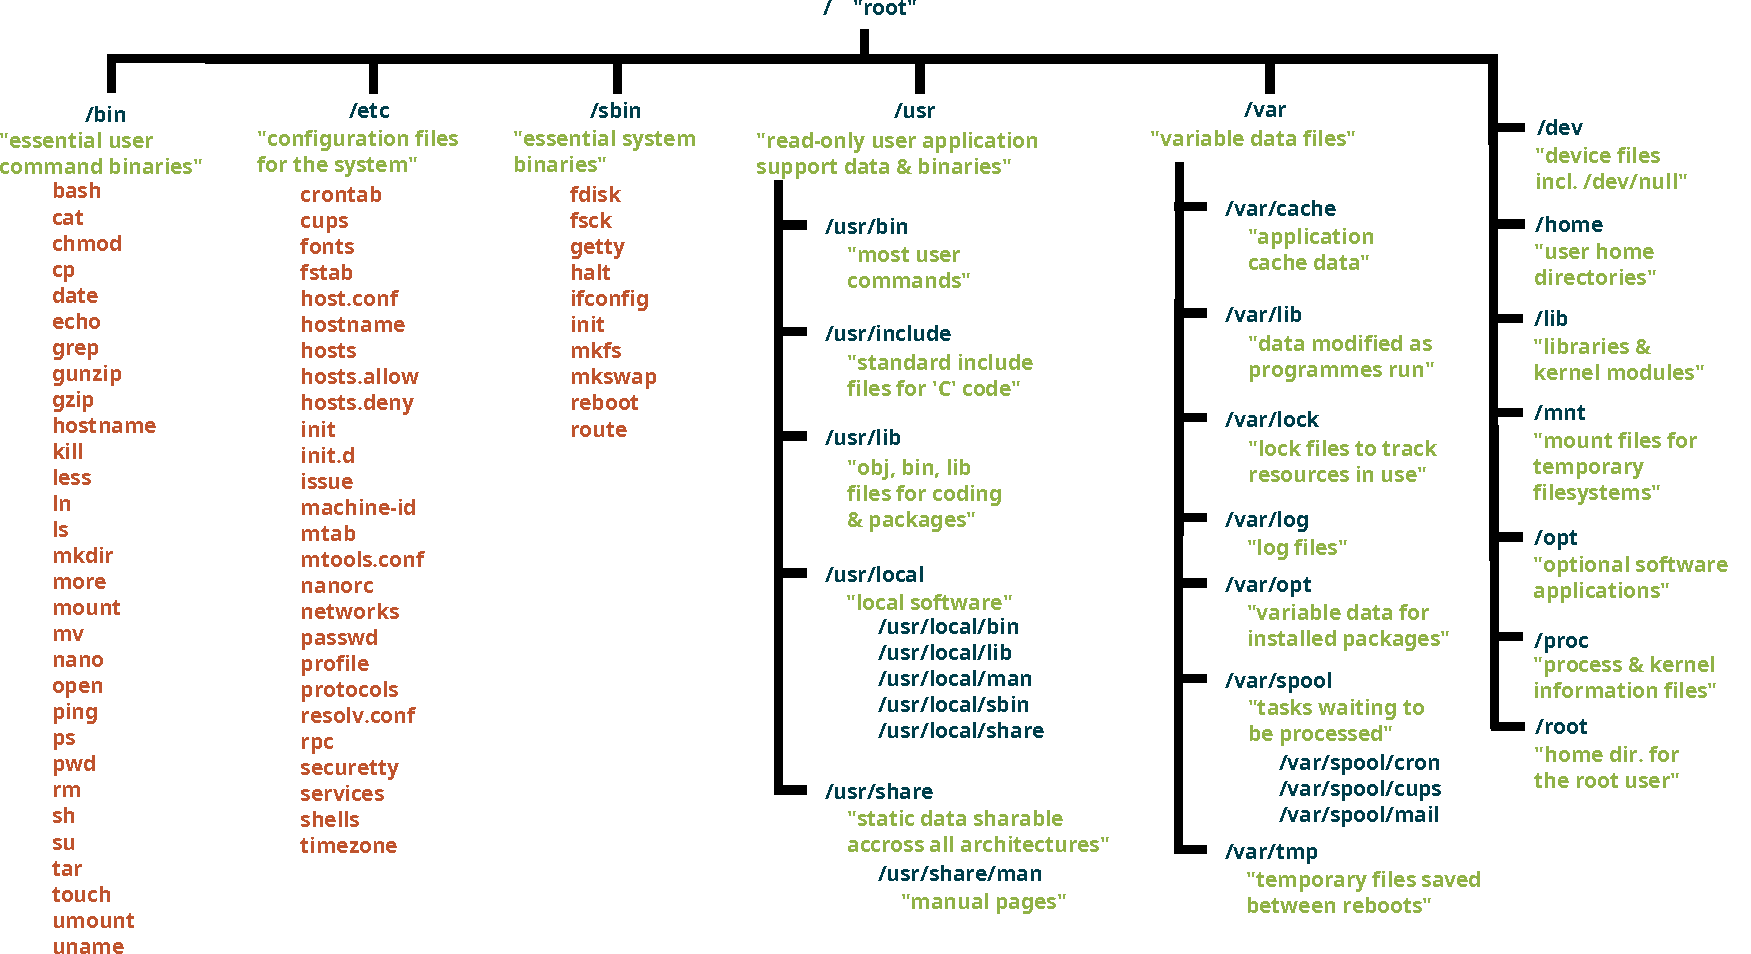
\includegraphics[width=0.9\textwidth]{res/Standard-unix-filesystem-hierarchy}
        \footnote{Quelle: https://commons.wikimedia.org/wiki/File:Standard-unix-filesystem-hierarchy.svg, Lizenz: CC-BY-SA-4.0}
    \end{center}
}

\frame{
    \frametitle{Literatur}
    \begin{itemize}
        \item https://collaboration.opengroup.org/external/pasc.org/plato/
        \item https://pubs.opengroup.org/onlinepubs/9699919799/utilities/contents.html
        \item http://sourceware.org/pthreads-win32/
        \item https://stackoverflow.com/questions/1780599/what-is-the-meaning-of-posix
        \item https://www.ibm.com/docs/en/watson-explorer/11.0.2?topic=queries-posix-regular-expression-syntax-examples
    \end{itemize}
}
\end{document}
